\documentclass[12pt]{article}
\usepackage{../../template}
\author{niceguy}
\title{Lecture 24}
\begin{document}
\maketitle

\section{Wave in an Open Channel}

A piston is pushing a body of fluid horizontally with velocity $\delta v$. Let $c_0$ be wavespeed, $y$ be depth, $\delta y$ be height of wave, and $b$ be width. Consider a control volume that moves with wavefront. As mass is conserved,

\begin{align*}
	\dot{m}_1 &= \dot{m}_2 \\
	\rho c_0 yb &= \rho(c_0-\delta V)(y+\delta y)b \\
	c_0\delta y &= \delta V(y + \delta y) \\
	\delta V &= c_0\frac{\delta y}{y + \delta y}
\end{align*}

Considering the momentum equation,

\begin{align*}
	\Delta F &= \dot{m}\Delta v \\
	\frac{1}{2}\rho g(y+\delta y)^2b - \frac{1}{2}\rho gy^2b &= \rho c_0yb\delta v \\
		g(1 + \frac{\delta y}{2y})\delta y &= c_0\delta v
\end{align*}

Combining both, we have

$$c_0^2 = gy(1+\frac{\delta y}{2y})(1+\frac{\delta y}{y})$$
Assuming $\delta y << y$, we have
$$c_0 = \sqrt{gy}$$

\begin{defn}
	The Froude number is
	$$\mathrm{Fr} = \frac{V}{\sqrt{gy}}$$
	When it is less than one, flow is subcritical. When it is equal to one, flow is critical. When it is greater than one, flow is supercritical.
\end{defn}

where $c_0$ is the wave speed and $y$ is the water depth.

\section{Compressible Flow}

Similarly, for sound waves, we have

\begin{align*}
	\dot{m}_\mathrm{in} &= \dot{m}_\mathrm{out} \\
	\rho cA &= (\rho+d\rho)(c-dv)A \\
	\rho c &= \rho c - \rho dv + cd\rho \\
	\rho dv &\approx cd\rho
\end{align*}

Using the momentum equation,

\begin{align*}
	(p+dp)A - pA &= \rho cAdv \\
	dp &= \rho cdv
\end{align*}

Combining,

$$c^2 = \left(\frac{\partial p}{\partial\rho}\right)_s$$

at constant $s$. \\
Under isentropic conditions,
$$\frac{p}{\rho^\gamma} = C$$
thus
$$c^2 = C\gamma\rho^{\gamma-1} = \gamma\frac{p}{\rho} = \gamma RT$$
for ideal gas, where the simplified equation
$$c = \sqrt{\gamma RT}$$
can be used. \\
More general, the bulk modulus
$$E_v = \frac{dp}{\frac{d\rho}{\rho}}$$
can be used, giving
$$c = \sqrt{\frac{E_v}{\rho}}$$

\begin{defn}
	The Mach number is defined as
	$$M = \frac{v}{c}$$
	where $c$ is the speed of sound in the same fluid. Flow is compressible only if the free stream Mach number $M_\infty > 0.3$.
\end{defn}

Similarly, we define subsonic, sonic and supersonic flow. We have transonic flow when $M \in [0.8,1]$ and hypersonic flow when $M \in [5,\infty)$.

\begin{ex}\label{continuity}
	Consider steady isentropic flow of 1D compressible flow.
	\begin{align*}
		\dot{m} &= C \\
		\rho vA &= 0 \\
		vAd\rho + \rho vdA + \rho Adv &= 0 \\
		\frac{d\rho}{\rho} + \frac{dA}{A} + \frac{dv}{v} &= 0
	\end{align*}
\end{ex}

\begin{ex}
	Steady Isentropic Flow of Compressible Flows

	\begin{figure}
		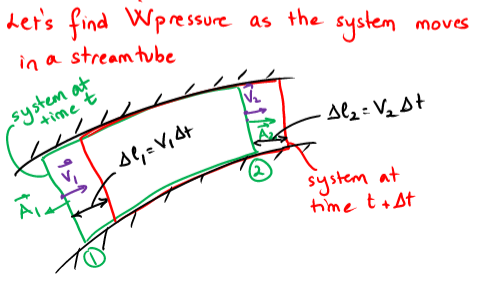
\includegraphics[width=0.7\textwidth]{stream.png}
		\caption{Work Done by Pressure}
	\end{figure}

	We first assume work done from friction is 0, and work done from shaft work is 0 under steady state. Work done by pressure is then
	\begin{align*}
		W &= W_1 + W_2 \\
		  &= p_1A_1v_1\Delta t - p_2A_2v_2\Delta t \\
		\dot{W} &= p_1A_1v_1 - p_2A_2v_2
	\end{align*}

	Using the Reynolds Transport Theorem,

	\begin{align*}
		\frac{dE_\mathrm{sys}}{dt} &= \frac{dE_\mathrm{cv}}{dt} + \dot{E}_\mathrm{out} - \dot{E}_\mathrm{in} \\
					   &= \dot{m}(e_2 + \frac{v_2^2}{2} + gz_2) - \dot{m}(e_1 + \frac{v_1^2}{2} + gz_2) \\
		p_1A_1v_1 - p_2A_2v_2 &= \dot{m}(e_2 + \frac{v_2^2}{2} + gz_2) - \dot{m}(e_1 + \frac{v_1^2}{2} + gz_2) \\
		\frac{p_2}{\rho_2} + e_2 + \frac{v_2^2}{2} + gz_2 &= \frac{p_1}{\rho_1} + e_1 + \frac{v_1^2}{2} + gz_1
	\end{align*}
	where $e_i$ is the internal energy at $i$. Substituting enthalpy,
	$$h_2 + \frac{v_2^2}{2} + gz_2 = h_1 + \frac{v_1^2}{2} + gz_1$$
\end{ex}

For high speed flows, the effect of height is negligible, hence
\begin{equation}\label{enth}
	h + \frac{v^2}{2} = C
\end{equation}

\begin{defn}
	We define \emph{stagnation enthalpy} as they enthalpy a fluid element achieves when it is brought to rest adiabetically.
	$$h_0 = h(v=0)$$
\end{defn}

Rewriting enthalpy in terms of specific heat and temperature,

\begin{align*}
	c_p(T-T_0) + \frac{v^2}{2} &= 0 \\
	T_0 &= T + \frac{v^2}{2c_p}
\end{align*}

Where $N_0$ denotes property $N$ at stagnation.

\begin{defn}
	The \emph{dynamic temperature} is defined as
	$$\Delta T = \frac{v^2}{2c_p}$$
\end{defn}

\begin{ex}
	The dynamic temperature of air at 100\unit{m.s^{-1}} is
	$$\Delta T = \frac{100^2}{2 \times 1.005\times10^3} = 5\unit{K}$$
	Therefore, air temperature rises by 5\unit{K} when it stagnates.
\end{ex}

Note that for low speed flow, temperature rise is negligible at stagnation. \\
Noting that $c_p = \frac{\gamma R}{\gamma-1}$,

\begin{align*}
	\frac{T_0}{T} &= 1 + \frac{(\gamma-1)v^2}{2\gamma RT} \\
		      &= 1 + \frac{(\gamma-1)v^2}{2c^2} \\
		      &= 1 + \frac{\gamma-1}{2}M^2
\end{align*}

Substituting isentropic relations
$$\frac{p_0}{p} = \left(\frac{\rho_0}{\rho}\right)^\gamma = \left(\frac{T_0}{T}\right)^{\frac{\gamma}{\gamma-1}}$$
we have
\begin{align*}
	\frac{p_0}{p} &= \left(\frac{\gamma-1}{2}M^2\right)^{\frac{\gamma}{\gamma-1}} \\
	\frac{\rho_0}{\rho} &= \left(\frac{\gamma-1}{2}M^2\right)^{\frac{1}{\gamma-1}}
\end{align*}

\begin{ex}
	Given $M_\infty = 2.2$ and $T_\infty = -30^\circ$C, find stagnation temperature.
	\begin{align*}
		\frac{T_0}{T} &= 1 + \frac{\gamma-1}{2}M^2 \\
		\frac{243}{T} &= 1 + \frac{1.4-1}{2}\times2.2^2 \\
		T &= 478\unit{K} \\
		  &= 205^\circ\text{C}
	\end{align*}
\end{ex}

\begin{ex}
	We consider flow incompressible when change in density is less than 5\%.
	\begin{align*}
		\frac{\rho_0}{\rho} &= \left(\frac{\gamma-1}{2}M^2\right)^{\frac{1}{\gamma-1}} \\
		1.05 &= \left(\frac{\gamma-1}{2}M^2\right)^{\frac{1}{1.4-1}} \\
		M &= 0.31
	\end{align*}
	Thus we consider flow to be incompressible when $M \leq 3$.
\end{ex}

Differentiating Equation~\ref{enth},
$$\frac{dp}{\rho} + vdv = 0$$
Combining with the continuity equation derived in \ref{continuity},

$$\frac{dA}{A} = -\frac{dv}{v}(1-M^2)$$

Therefore, at subsonic flow, $\frac{dA}{dv} < 0$, and at supersonic flow, $\frac{dA}{dv} > 0$, where flow accelerates as area increases.

\end{document}
